% Source: https://tex.stackexchange.com/a/648913/6880

\documentclass{beamer}

%layout
\mode<presentation>{
\usetheme{Madrid}
}
\usepackage{tikz}
\usetikzlibrary{fit}

\begin{document}
    \begin{frame}
        \begin{center}
            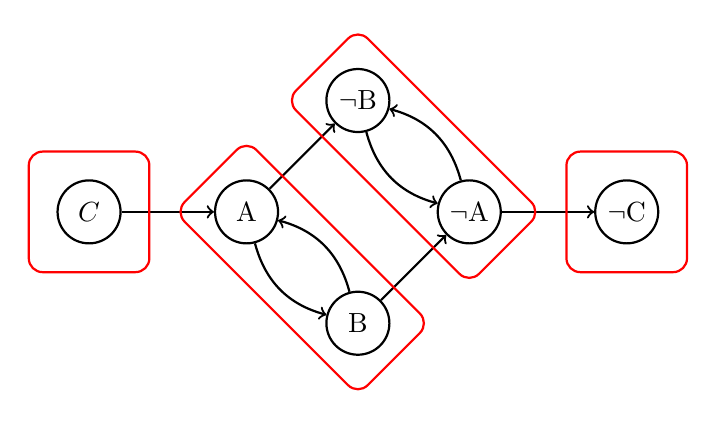
\begin{tikzpicture}[
                node distance={20mm},
                thick,
                main/.style = {draw, circle, inner sep=2pt, minimum size=8mm},
                box/.style = {draw,red,inner sep=10pt,rounded corners=5pt}] 
                
                \node[main] (1) {$C$}; 
                \node[main] (2) [right of=1] {A}; 
                \node[main] (3) [below right of=2] {B}; 
                \node[main] (4) [above right of=2] {$\neg$B}; 
                \node[main] (5) [below right of=4] {$\neg$A}; 
                \node[main] (6) [right of=5] {$\neg$C};
                \draw[->] (1) -- (2);
                \draw[->] (2) to [bend right=30] (3);
                \draw[->] (2) -- (4);
                \draw[->] (3) to [bend right=30](2);
                \draw[->] (3) -- (5);
                \draw[->] (4) to [bend right=30] (5);
                \draw[->] (5) to [bend right=30] (4);
                \draw[->] (5) -- (6);
            
                \node[box,fit=(1)] {};
                \node[box,rotate fit=45,fit=(2)(3)] {};
                \node[box,rotate fit=45,fit=(4)(5)] {};
                \node[box,fit=(6)] {};
            \end{tikzpicture} 
        \end{center}
    \end{frame}
\end{document}